\chapter{Medical Fundamentals}
Comprehension of the physiological functionality of the human heart and the cardiovascular system is an important prerequisite to the work addressed in this thesis. Therefore the basics of these topics will be explained in this chapter.

\section{Cardiovascular System}
The fundamental task of the cardiovascular system is to supply all organs with blood. The system, is divided into two components. The systemic circulation and the pulmonary circulation. As shown in Figure \ref{fig:circulation}, which represents the percentage distribution of the blood over the circulatory system, the systemic circulation is supplying blood flow to all tissues and organs except the lung. Due to this it is also referred to as the greater circulation. \cite{GH20}
\begin{figure}[h]
  \centering
  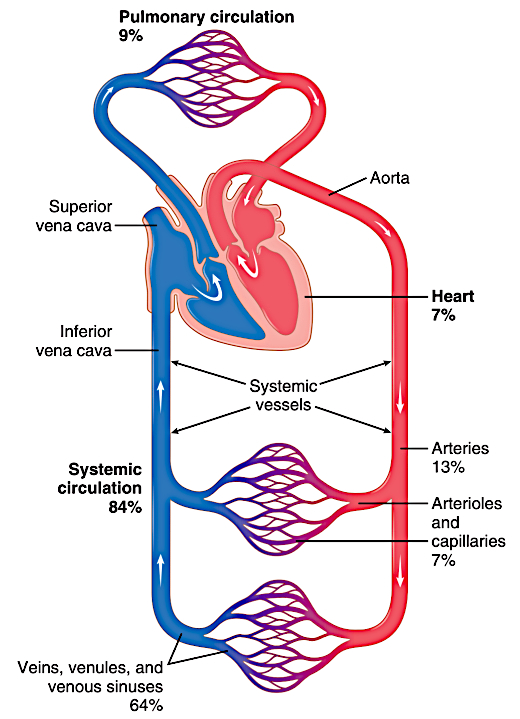
\includegraphics[width=0.4\textwidth, height=0.6\textwidth]{images/circulation.jpg}
  \caption{Blood distribution in the circulatory system \cite{GH20}.}
  \label{fig:circulation}
\end{figure}
 The center of the circulatory system is the heart. The heart itself consists of two mechanical pumps, which are functionally connected in series, but are united in one organ. It is separated into two sides, which themselves are divided into an atrium and a ventricle. The atria act as weak primer pumps, needed to provide blood flow to the ventricles.\cite{HKS4} Both the atrium and the ventricle are surrounded by the myocardium, which acts as the working muscle of the heart. Through the contraction of the myocardium blood is pumped into the circulatory system.\cite{HKS7} The left ventricle is pumping oxygenated blood through the aorta into the systemic circulation. There, the oxygen stored in the blood is delivered to the organs. The blood, now low in oxygen, is then led into the right atrium through the inferior and superior vena cava. From the right atrium, the deoxygenated blood then enters the right ventricle and then the pulmonary circulation via the pulmonary artery. After the blood is oxygenated in the lungs, it is returned to the left atrium through the pulmonary vein.\cite{HKS4} In addition to the atria and the ventricles each side of the heart has an atrioventricular (AV) valve, as well as a semilunar (SL) valve. The AV valve of the left heart is called mitral valve, the one of the right heart is the tricuspid valve. The aortic valve and pulmonary valve are the SL valves of the left and right heart, respectively.\cite{HKS7} Figure \ref{fig:heart_anat} provides a graphic overview on the anatomy of the heart and the course of blood flow through the heart. The amount of blood pumped through the two sides of the heart is equal. This value is called cardiac output (CO). It is calculated through the multiplication of the heart rate (HR) and the stroke volume (SV). For an average adult at rest, with a heart rate of approximately $70 min^{-1}$ and a stroke volume of 70 ml this leads to
 \begin{equation}
   CO = HR \times SV = 70 min^{-1} \times 70ml = 5 \frac{l}{min}
  \label{eq:CO}
 \end{equation}
In case of maximum physical load the cardiac output can increase as high as $20\frac{l}{min}$, for a stroke volume of 110 ml and a heart rate of $190 min^{-1}$. \cite{HKS4}

\begin{figure}
  \centering
  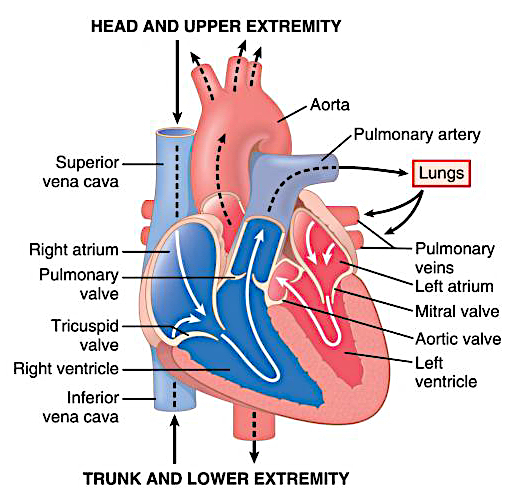
\includegraphics[width=0.6\textwidth]{images/heart_1.jpg}
  \caption{Anatomy of the human heart \cite{GH20}.}
  \label{fig:heart_anat}
\end{figure}

\\The cardiac cycle describes the events that occur during the time-span of one heartbeat. It is triggered by an electrochemical action potential originating from the sinus node. The cycle is divided into four phases. Figure \ref{fig:cardiac_cycle} illustrates these action phases and events of the cardiac cycle for the left ventricle. During the period of isovolumic contraction the  ventricular pressure increases. For the left ventricle the pressure increases from about 4-6 mmHg to 80 mmHg. The values for the right ventricle are much lower. This increase is happening as a direct result of the ventricular contraction. The AV valves as well as the SL valve are closed during this process. This leads to a constant blood volume in the ventricles. As soon as the ventricular pressure exceeds the arterial pressure the pulmonary and aortic valves open and blood is able to flow into the aorta and the pulmonary artery. This phase is called ejection phase, as the blood is ejected into the circulatory system. During this phase the blood volume in the ventricle decreases by 55-60\%. The ventricular pressure keeps increasing for a while due to the contraction of the myocardium, before decreasing as the relaxation of the myocardium sets in. The period of isovolumic contraction in combination with the ejection phase is called systole. 
\begin{figure}[h]
  \centering
  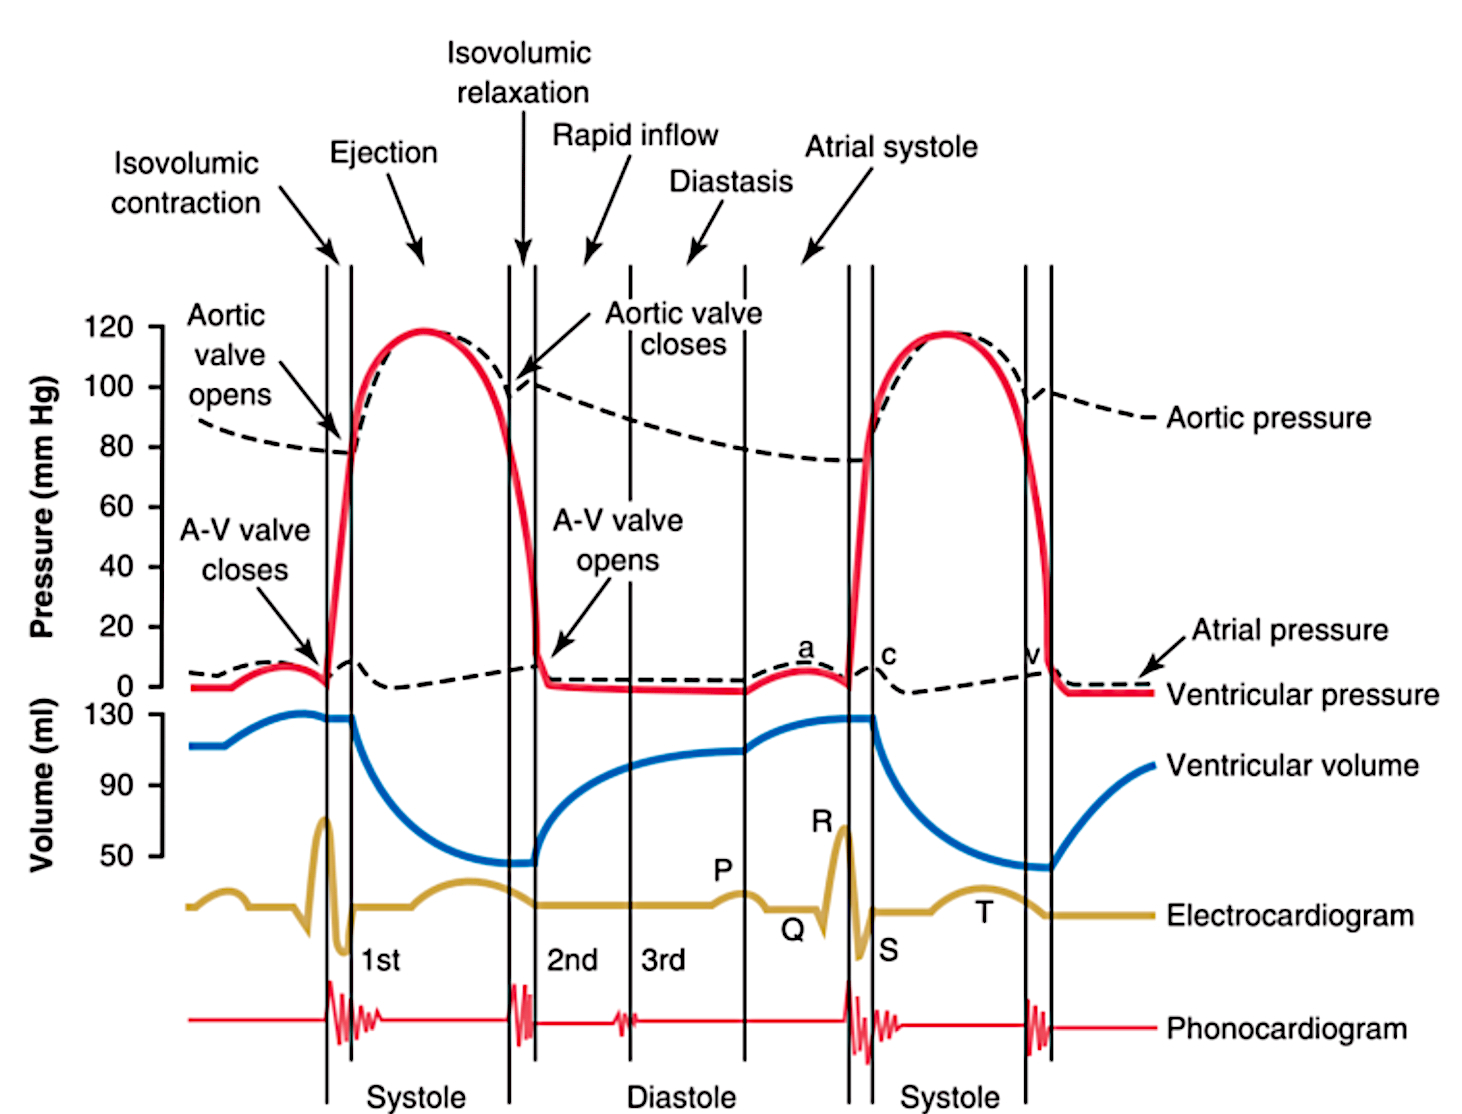
\includegraphics[width=0.8\textwidth]{images/cardiac_cycle.jpg}
  \caption{Action phases of the cardiac cycle based on the example of the left ventricle \cite{GH20}.}
  \label{fig:cardiac_cycle}
\end{figure}
\section{Heartinsufficency}
